\subsection{Computer Vision Implementation} \label{compvis_implementation}

    Both the thermal and radar Computer Vision (CV) models are implemented using Ultralytics YOLOv11\footnote{\url{https://github.com/ultralytics/ultralytics}}—a state-of-the-art, real-time object detection framework based on convolutional neural networks (CNNs). The software is free and open source, and released under a copyleft license\footnote{\url{https://github.com/ultralytics/ultralytics/blob/main/LICENSE}}. Although both systems utilise YOLOv11, there are significant differences in their network architectures and, notably, in the characteristics of their training, validation and testing datasets.


\subsubsection{Datasets Comparison} \label{sec:cv_dataset_comparison}

The thermal dataset consists of 1,080 images sourced from Roboflow\footnote{\url{https://universe.roboflow.com/xamurani/landmines_detection}}, captured from altitudes between 1 and 10\,m, with mines of a wide variety, and buried between 0 and 5\,cm deep. This diversity allows the network to learn robust and generalisable features. In contrast, the radar dataset, again sourced from Roboflow\footnote{\url{https://universe.roboflow.com/hassan-sdqop/gpr-data-n3n5u}} comprises only 100 raw B-scans generated from simulated data. These B-scans are extremely \textit{'clean'}, and lack noisy effects caused by real-world conditions such as soil heterogeneity, surface roughness and vegetation, that would be seen by an operational radar sensor. The effect of soil heterogeneity on the radar B-scans is investigated in Section \ref{compvis_radarsims}. 

\begin{figure}[htbp]
  \centering
  \begin{subfigure}[t]{0.48\textwidth}
    \centering
    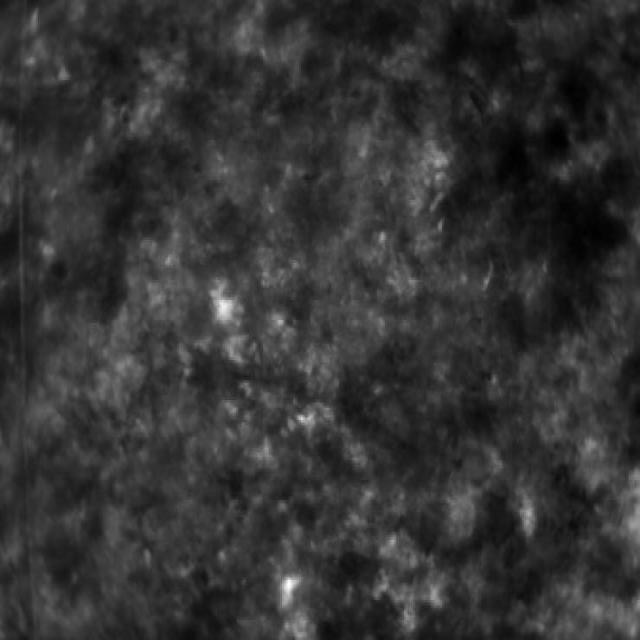
\includegraphics[width=\textwidth]{figs/Rory/A_thermal_image.jpg} % Thermal example
    \caption{Thermal Dataset Example}
    \label{fig:thermal_example}
  \end{subfigure}
  \hfill
  \begin{subfigure}[t]{0.48\textwidth}
    \centering
    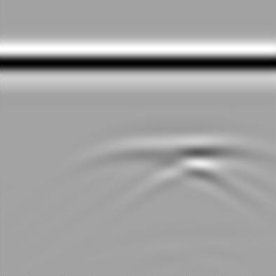
\includegraphics[width=\textwidth]{figs/Rory/A_radar_image.jpg} % Radar example
    \caption{Radar Dataset Example}
    \label{fig:radar_example}
  \end{subfigure}
  \caption{Example Images from Thermal and Radar Datasets}
  \label{fig:dataset_examples}
\end{figure}

\subsubsection{Architecture Comparison} \label{sec:cv_architecture_comparison}

Both models are built on the YOLOv11 Large model\footnote{\url{https://github.com/ultralytics/ultralytics}}, which prescribes the final network architecture; the thermal model results in a deeper network with 464 layers and 25,280,083 parameters, while the radar model, despite having the same parameter count, is shallower, with only 190 layers. This difference likely reflects the greater complexity required to extract features from the diverse thermal images, compared to the more uniform raw radar B-scans. For more detail of the YOLOv11 model, see \cite{khanam2024yolov11}

\subsubsection{Training} \label{sec:cv_training_comparison}


\begin{wrapfigure}{r}{0.35\textwidth} % Align right, width = 0.48\textwidth
  \centering
  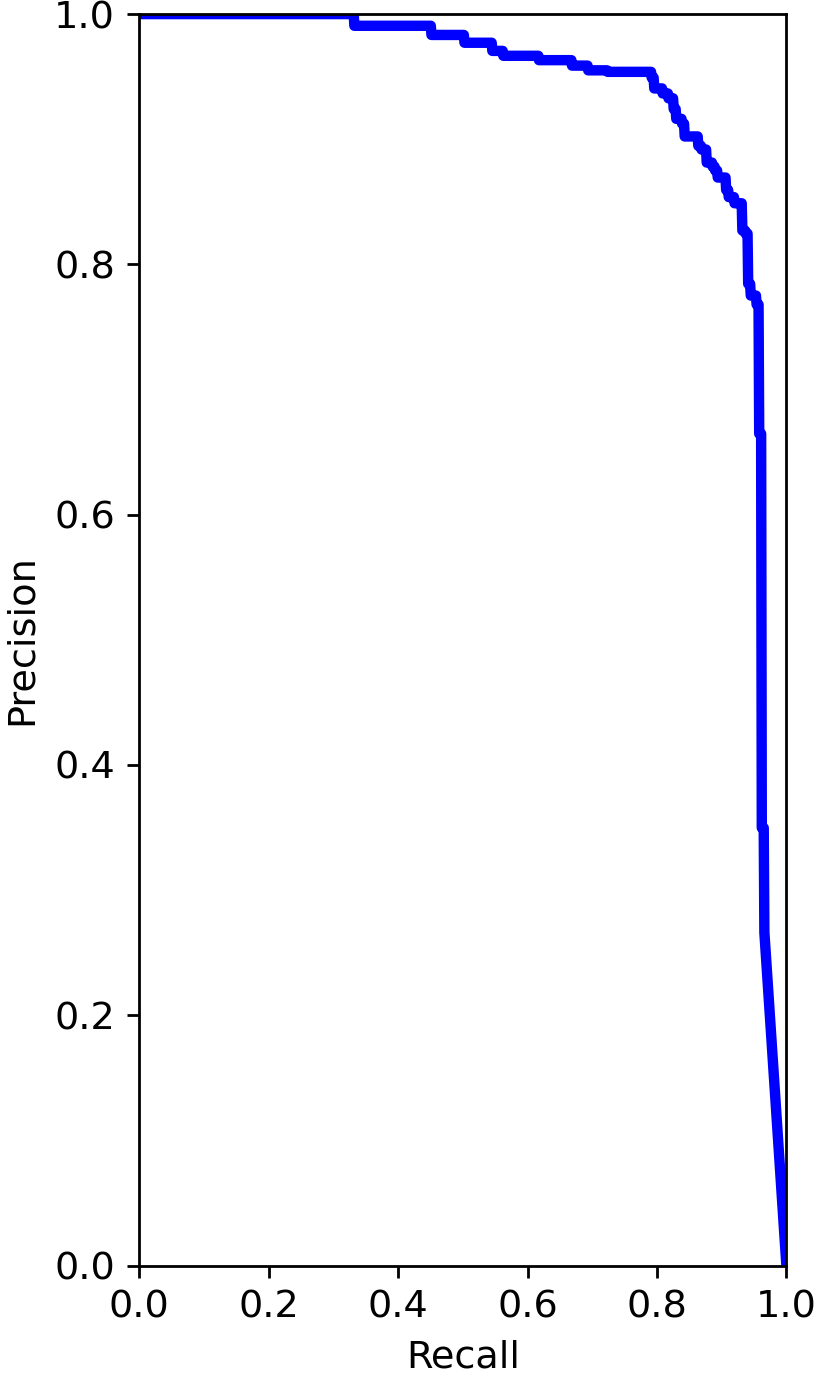
\includegraphics[width=\linewidth]{figs/Rory/APR_curve_therm.png} % Use \linewidth to match wrapfig width
  \caption{Precision-Recall (PR) curve for the thermal YOLOv11 model}
  \label{fig:pr_curve}
\end{wrapfigure}

The thermal model was trained for 100 epochs on a Tesla T4 GPU via Google Colab, taking 1.153 hours. The per-image average processing times were 1.3\,ms (preprocessing), 14.9\,ms (inference), and 3.6\,ms (postprocessing). In contrast, the radar model, also trained for 100 epochs on a T4 GPU, completed training in just 0.156 hours, with average processing times of 0.2\,ms (preprocessing), 10.2\,ms (inference), and 1.0\,ms (postprocessing). The 30\% faster inference time and 86\% faster training time for the radar model is a reflection of the radar dataset's limited size and diversity.

\subsubsection{Results} \label{sec:cv_results_comparison}

Due to the limited variability of the radar training set, the radar models' performance statistics were high. The optimal confidence threshold of 0.405 was chosen (maximising the F1 score \footnote{\url{https://www.v7labs.com/blog/f1-score-guide}}), yielding a precision of 97.6\% and a recall of 100\% on unseen data.

Despite the significant diversity of the thermal dataset, the thermal model performed well. The precision-recall curve is visualised in Figure \ref{fig:pr_curve}, demonstrating that high precision can be maintained across a large range of recall values. The trade-off between precision and recall is discussed in Section \ref{lossmatrix}, where it is argued that recall for the thermal sensor should be maximised, with precision as a secondary consideration. Therefore optimisation is not as simple as maximising the F1 score, and instead the optimal confidence threshold was selected manually as 0.299, yielding a precision of 85.1\% and a recall of 91.9\% on unseen data. The results are summarised in Table \ref{tab:sensor_comparison}.

\begin{table}[htbp]
\centering
\caption{Comparison of Thermal and Radar Sensor Performance}
\label{tab:sensor_comparison}
\begin{tabular}{lcc}
\hline
\textbf{Metric} & \textbf{Thermal} & \textbf{Radar} \\ 
\hline
Dataset size & 1,020 & 100 \\
Train:Val:Test split & 70:15:15 & 70:15:15 \\
Dataset variability & highly varied & not at all varied \\
CNN architecture & YOLOv11 Large & YOLOv11 Large \\
Number of layers & 464 & 190 \\
Number of parameters & 25280083 & 25280083 \\
Optimiser & Adam & Adam \\
Training Hardware & T4 GPU\footnote{\label{ftn:t4gpu}NVIDIA Tesla T4 GPU} & T4 GPU\\
Training time (100 epochs) & 1.153\,hr & 0.156\,hr \\
Inference time & 14.9\,ms & 10.2\,ms \\
Image type & Thermal Images & Raw B-scans \\
Chosen confidence threshold & 0.299 & 0.405 \\
\hline
\rowcolor{gray!10} \textbf{Precision} & \textbf{85.1\%} & \textbf{97.6\%} \\
\rowcolor{gray!10} \textbf{Recall} & \textbf{91.9\%} & \textbf{100\%} \\
\hline
\end{tabular}
\end{table}


    \subsubsection{Class Imbalance} \label{class_imbalance}

        \noindent The thermal and radar training datasets contain only images of landmines (100\% positive samples), whereas in real-world scenarios, a deployed CNN would encounter one the order of 1\%. This discrepancy introduces a \textit{class imbalance}, where networks trained exclusively on positive samples lack exposure to "safe" regions, leading to elevated false positive rates. To mitigate this, Section~\ref{fusion_bounds} applies Bayesian posterior densities (\(\rho_1, \rho_2\)) derived from a prior mine density, rather than relying on the raw precision metrics. This approach addresses the \textit{accuracy paradox}\footnote{\url{https://en.wikipedia.org/wiki/Accuracy_paradox}}.

        \noindent Although physics-informed fusion (Section~\ref{ANFIS}) mitigates imbalance effects, training on balanced datasets would further close the gap between theoretical upper bounds and real-world performance. Therefore future work should explore training on datasets with realistic mine densities (1-5\% positive samples).

        
    \subsubsection{Justification for Simulations} \label{simulation_justification}
    
    
        \paragraph{Thermal} 
        
            
           It was shown in Section \ref{sec:cv_results_comparison} that the thermal computer vision model performs well on an unseen dataset of highly varied images. This means the model can extract general 'landmine' features, and that \textit{given some features can be resolved by the sensor}, the model is likely to be able to detect them. Therefore, provided the peak temperature difference between the ambient soil and the soil directly above a buried landmine, denoted \(\Delta T\), is significantly greater than the sensitivity of the thermal sensor, which is 0.05\,K (see Section \ref{hardware}), then the thermal model will be able to detect the landmine. This is the \textbf{detectability hypothesis}.

            It has been shown by Van Dam et al. \cite{van2003effects} that the most challenging environmental conditions for thermal detection are dry and hot conditions, where the lowest measurable \(\Delta T\) will occur. This is validated in Section \ref{sec:cv_sensitivity}. Therefore, it suffices to simulate the thermal return from a landmine buried in Afghanistan, where it is hot, and the soils are sandy, to validate that the thermal detection system will work in even the most challenging environmental conditions. Afghanistan is also relevant because it is one of the most densely mined countries in the world, with a large body of humanitarian work in the area.
        
        \paragraph{RADAR} 

            \noindent The motivation behind the radar computer vision simulations is clear. The publicly available datasets are so limited in their diversity and size that they may not be useful for training models to detect landmines in real, noisy B-scans. B-scans need to be produced in simulation using as few assumptions as possible, attempting to replicate some of the physical noise-generating processes, as opposed to solely adding statistical noise to a 'clean' B-scan. In Section \ref{compvis_radarsims}, the effect of heterogeneous soil variability is investigated. This has not been thoroughly investigated in literature, as noted by Van Dam et al. \cite{van2003effects}: \textit{“The important role of soil variability has hardly been systematically studied.”}
            This would allow for validation of whether the model is robust to noise not represented in its training data. If it is, then a more advanced model trained on real experimental data would outperform this model significantly, and be effective in operation.
    
    
    